\documentclass[a4paper, 12pt]{article}
\usepackage[a4paper,top=1.5cm, bottom=1.5cm, left=1cm, right=1cm]{geometry}
\usepackage{cmap}
\usepackage{mathtext}
\usepackage[T2A]{fontenc}
\usepackage[utf8]{inputenc}
\usepackage[english,russian]{babel}
\usepackage{multirow}
\usepackage{graphicx}
\usepackage{wrapfig}
\usepackage{tabularx}
\usepackage{float}
\usepackage{wrapfig}
\usepackage{longtable}
\usepackage{booktabs}
\usepackage{hyperref}
\hypersetup{colorlinks=true,urlcolor=blue}
\usepackage[rgb]{xcolor}
\usepackage{amsmath,amsfonts,amssymb,amsthm,mathtools}
\usepackage{icomma}
\usepackage{euscript}
\usepackage{mathrsfs}
\usepackage{enumerate}
\usepackage{caption}
\usepackage{mathtools}
\usepackage[]{esdiff}
\mathtoolsset{showonlyrefs=true}
\usepackage{subcaption}
\usepackage[europeanresistors, americaninductors]{circuitikz}
\DeclareMathOperator{\sgn}{\mathop{sgn}}
\newcommand*{\hm}[1]{#1\nobreak\discretionary{}
	{\hbox{$\mathsurround=0pt #1$}}{}}

\begin{document}

\begin{center}
    \huge
    \bf{Лабораторная работа 3.4.1.}

    \bf{Диа- и парамагнетики}

    \bf{Солодилов Михаил Б01-306}
\end{center}

\begin{center}
    \section*{Введение}
\end{center}

\noindent \textbf{Цель работы:}
измерение магнитной восприимчивости диа- и парамаг­нитного образцов.

\bigskip

\noindent \textbf{Оборудование:}
электромагнит, аналитические весы, милливе­
берметр, регулируемый источник постоянного тока, образцы.

\centering
\begin{tabular}{|c|c|c|}
    \toprule
    Материал & $m$, мг & $d$, см \\
    \midrule
    Al & 25255 & 1.0 \\
    \midrule
    Cu & 83170 & 1.0 \\
    \bottomrule
\end{tabular}

\bigskip

\subsection*{Экспериментальная установка}

\begin{figure}[H]
    \centering
    \begin{subfigure}{0.9\textwidth}
        \centering
        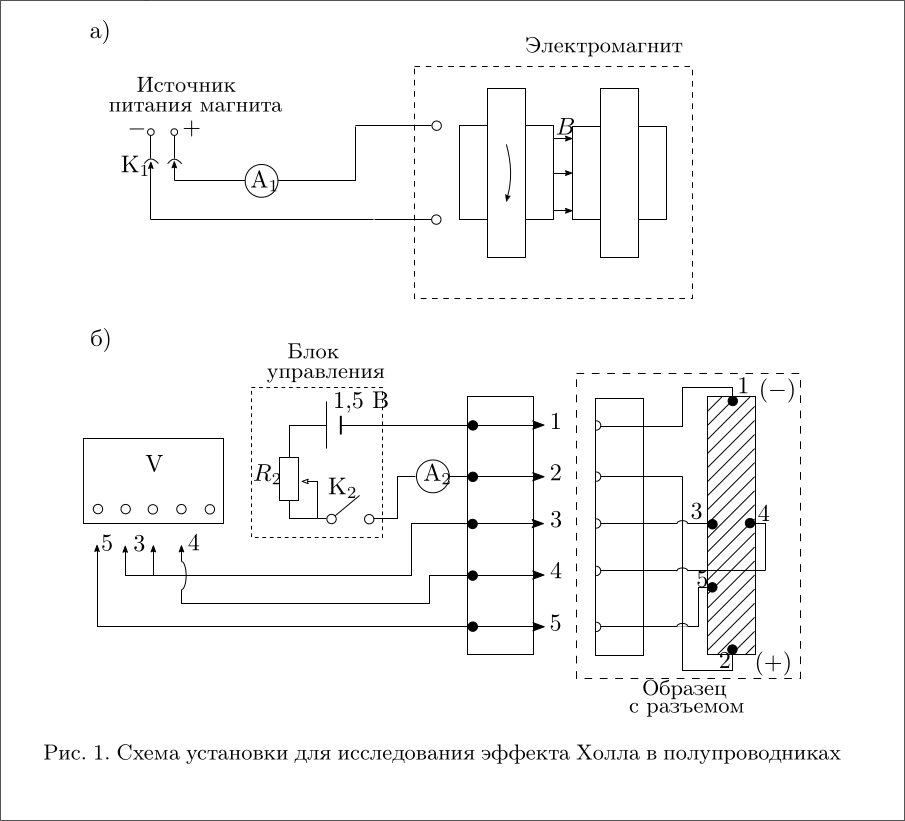
\includegraphics[width=1\textwidth]{img/Setup.png}
    \end{subfigure}
\end{figure}

\raggedright
Схема установки изображена на рисунке. Магнитное поле с максимальной индукцией
$\approx 1$ Тл создаётся в зазоре электромагнита, питаемого
постоянным током. Диаметр полюсов существенно превосходит шири­ну зазора,
поэтому поле в средней части зазора достаточно однородно.
Величина тока, проходящего через обмотки электромагнита, задаётся
регулируемым источником постоянного напряжения.

\newpage

\centering
\subsection*{Работа}

\raggedright

Для начала проградуируем магнит.

\begin{table}[htbp]
    \centering
    \begin{tabular}{|c|c|}
    \hline
    $I, \, \text{А}$ & $B, \, \text{Тл}$ \\ \hline
    $ 0.33 $ & $ 0.1263 $ \\ \hline
    $ 0.75 $ & $ 0.2404 $ \\ \hline
    $ 1.25 $ & $ 0.3761 $ \\ \hline
    $ 1.50 $ & $ 0.4440 $ \\ \hline
    $ 1.85 $ & $ 0.5390 $ \\ \hline
    $ 2.25 $ & $ 0.6476 $ \\ \hline
    $ 2.62 $ & $ 0.7480 $ \\ \hline
    $ 3.05 $ & $ 0.8648 $ \\ \hline
    \end{tabular}
    \caption{Градуировка}
\end{table}

\begin{figure}[H]
   \centering
   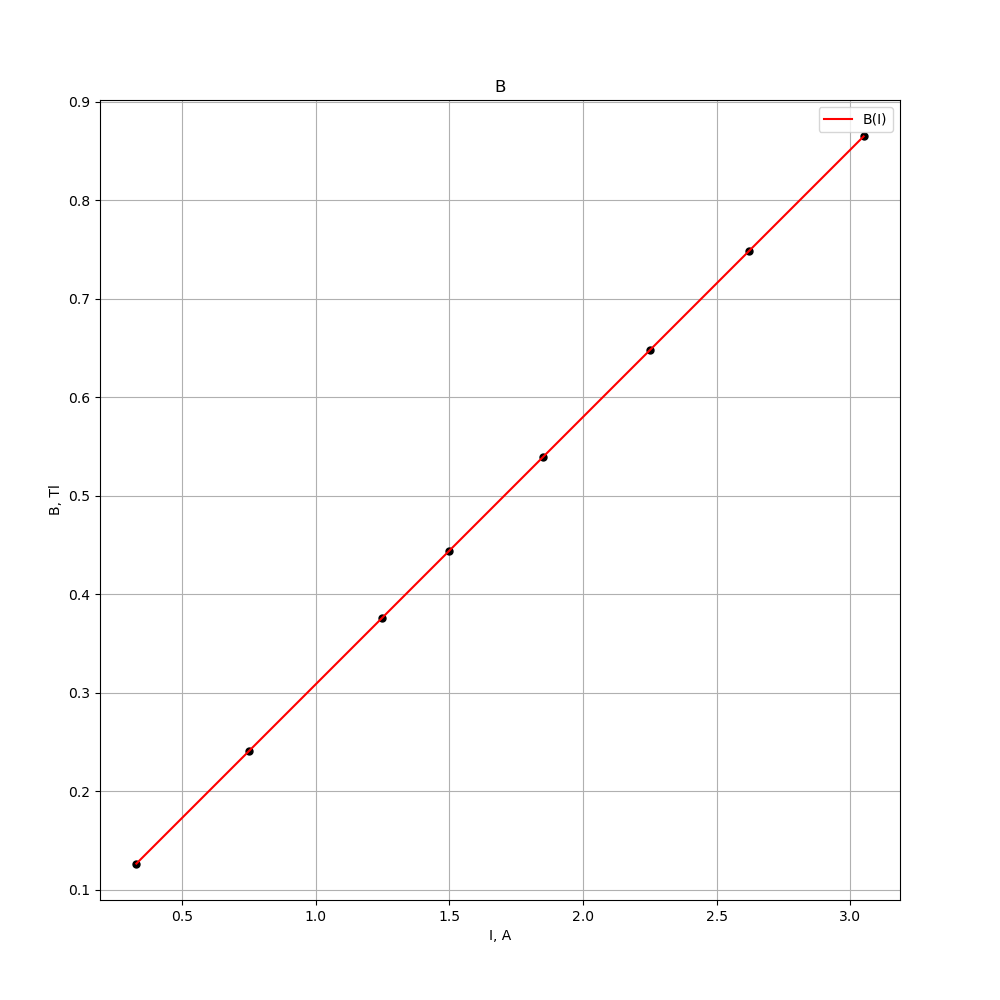
\includegraphics[width=0.8\textwidth]{img/B(I).png}
   \caption{$B(I)$}
\end{figure}

\begin{figure}[H]
    \centering
    \begin{minipage}{0.5\textwidth}
        \centering
        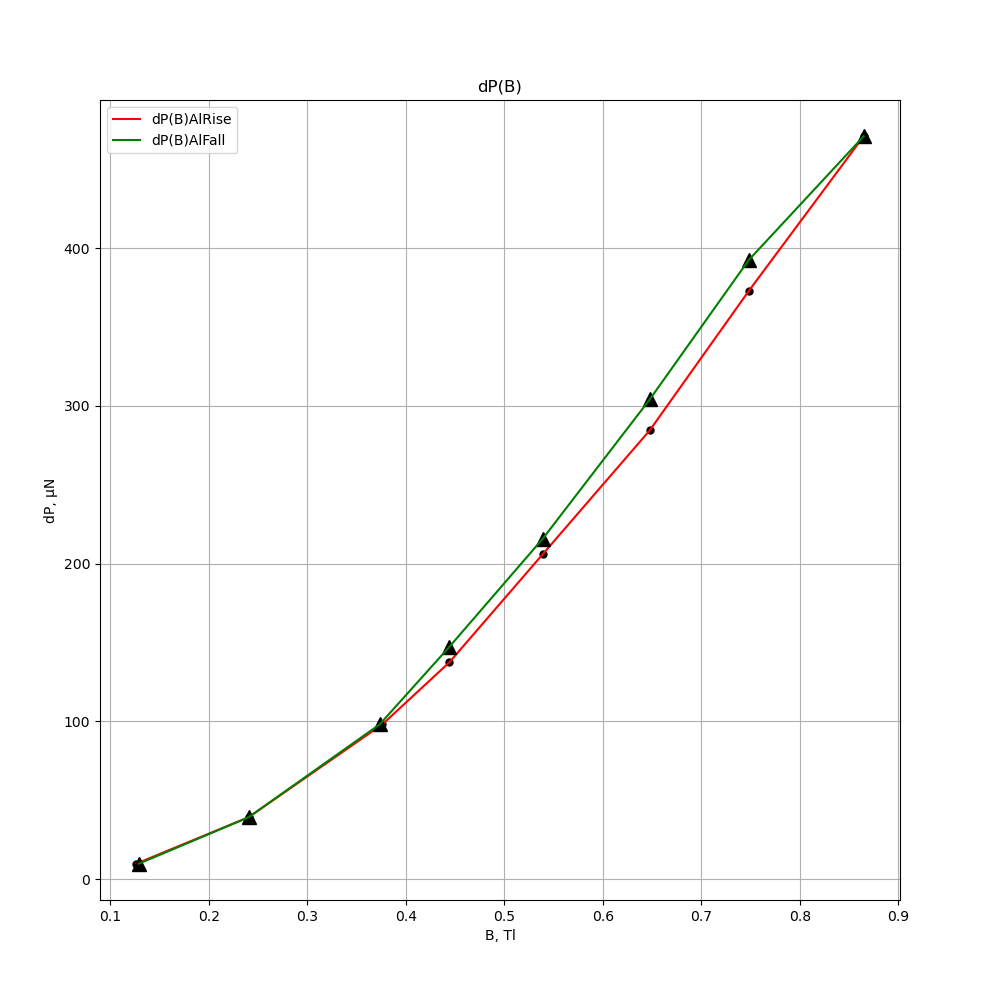
\includegraphics[width=\textwidth]{img/dP(B)Al.png}
        \caption{Al}
        \label{fig:image1}
    \end{minipage}\hfill
    \begin{minipage}{0.5\textwidth}
        \centering
        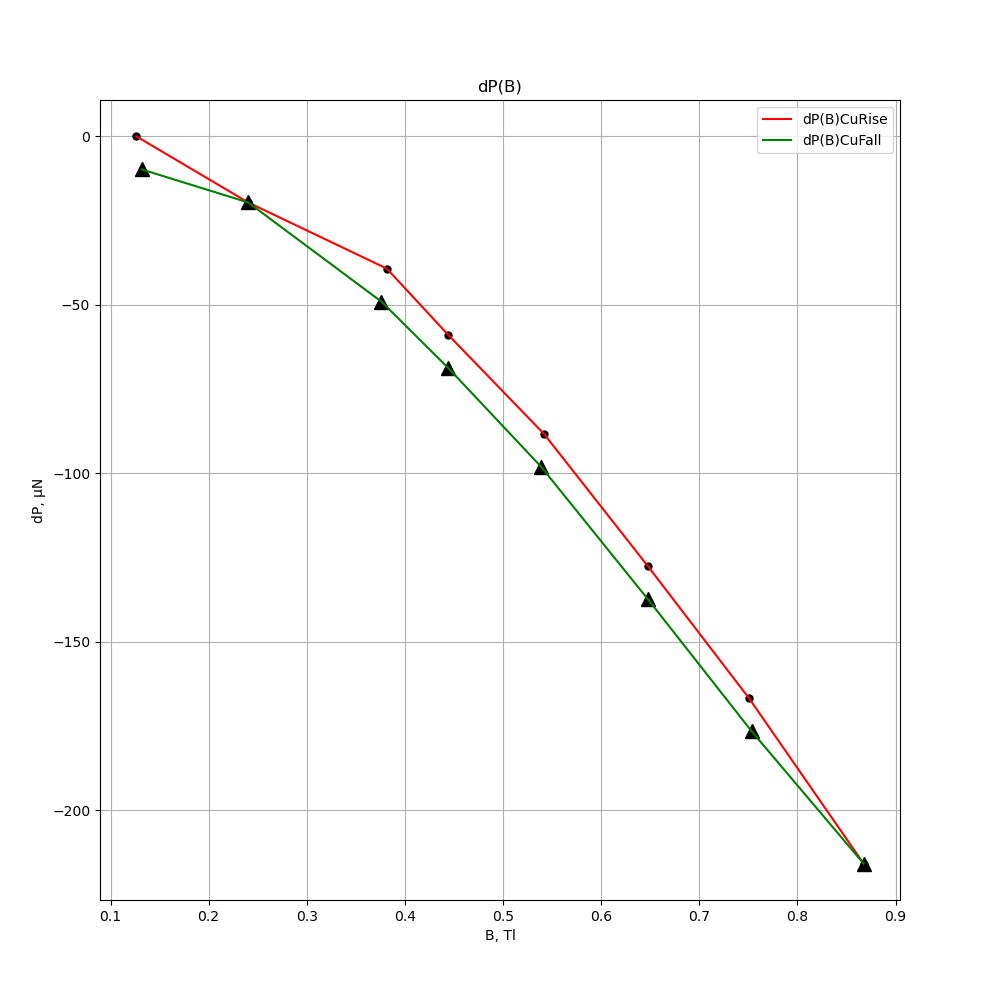
\includegraphics[width=\textwidth]{img/dP(B)Cu.png}
        \caption{Cu}
        \label{fig:image2}
    \end{minipage}
\end{figure}

Как мы можем увидеть, алюминий является парамагнетиком, так как он втягивается
в магнит, а медь - диамагнетика, потому что выталкивается.

\begin{table}[htbp]
    \centering
    \begin{subtable}[t]{0.45\textwidth}
        \centering
        \begin{tabular}{|c|c|c|c|}
        \hline
        \multicolumn{2}{|c|}{Al} & \multicolumn{2}{c|}{Cu} \\ \hline
        $dP, \mu N$ & $B, Tl$ & $dP, \mu N$ & $B, Tl$      \\ \hline
        9.81   & 0.12 & 0       & 0.12  \\ \hline
        39.24  & 0.24 & -19.62  & 0.24  \\ \hline
        98.10  & 0.37 & -39.24  & 0.38  \\ \hline
        137.34 & 0.44 & -58.86  & 0.44  \\ \hline
        206.01 & 0.53 & -88.29  & 0.54  \\ \hline
        284.49 & 0.64 & -127.53 & 0.64  \\ \hline
        372.78 & 0.74 & -166.77 & 0.75  \\ \hline
        470.88 & 0.86 & -215.82 & 0.86  \\ \hline
        470.88 & 0.86 & -215.82 & 0.86  \\ \hline
        392.40 & 0.74 & -176.58 & 0.75  \\ \hline
        304.11 & 0.64 & -137.34 & 0.64  \\ \hline
        215.82 & 0.53 & -98.10  & 0.53  \\ \hline
        147.15 & 0.44 & -68.67  & 0.44  \\ \hline
        98.10  & 0.37 & -49.05  & 0.37  \\ \hline
        39.24  & 0.24 & -19.62  & 0.24  \\ \hline
        9.81   & 0.12 & -9.81   & 0.13  \\ \hline
        \end{tabular}
        \caption{$dP(B)$ для Al и Cu}
    \end{subtable}%
    \hfill
    \begin{subtable}[t]{0.45\textwidth}
        \centering
        \begin{tabular}{|c|c|c|c|}
        \hline
        \multicolumn{2}{|c|}{Al} & \multicolumn{2}{c|}{Cu} \\ \hline
        $dP, \mu N$ & $B^2, Tl^2$ & $dP, \mu N$ & $B^2, Tl^2$      \\ \hline
        9.81   & 0.0160  & 0      & 0.0160  \\ \hline
        39.24  & 0.0578  & -19.62 & 0.0578  \\ \hline
        98.10  & 0.1415  & -39.24 & 0.1456  \\ \hline
        137.34 & 0.1971  & -58.86 & 0.1971  \\ \hline
        206.01 & 0.2905  & -88.29 & 0.2934  \\ \hline
        284.49 & 0.4194  & -127.53 & 0.4194  \\ \hline
        372.78 & 0.5595  & -166.77 & 0.5636  \\ \hline
        470.88 & 0.7478  & -215.82 & 0.7525  \\ \hline
        470.88 & 0.7478  & -215.82 & 0.7525  \\ \hline
        392.40 & 0.5595  & -176.58 & 0.5677  \\ \hline
        304.11 & 0.4194  & -137.34 & 0.4194  \\ \hline
        215.82 & 0.2905  & -98.10  & 0.2905  \\ \hline
        147.15 & 0.1971  & -68.67  & 0.1971  \\ \hline
        98.10  & 0.1394  & -49.05  & 0.1415  \\ \hline
        39.24  & 0.0578  & -19.62  & 0.0578  \\ \hline
        9.81   & 0.0167  & -9.81   & 0.0174  \\ \hline
        \end{tabular}
        \caption{$dP(B^2)$ для Al и Cu}
    \end{subtable}
\end{table}

\begin{figure}[H]
    \centering
    \begin{minipage}{0.5\textwidth}
        \centering
        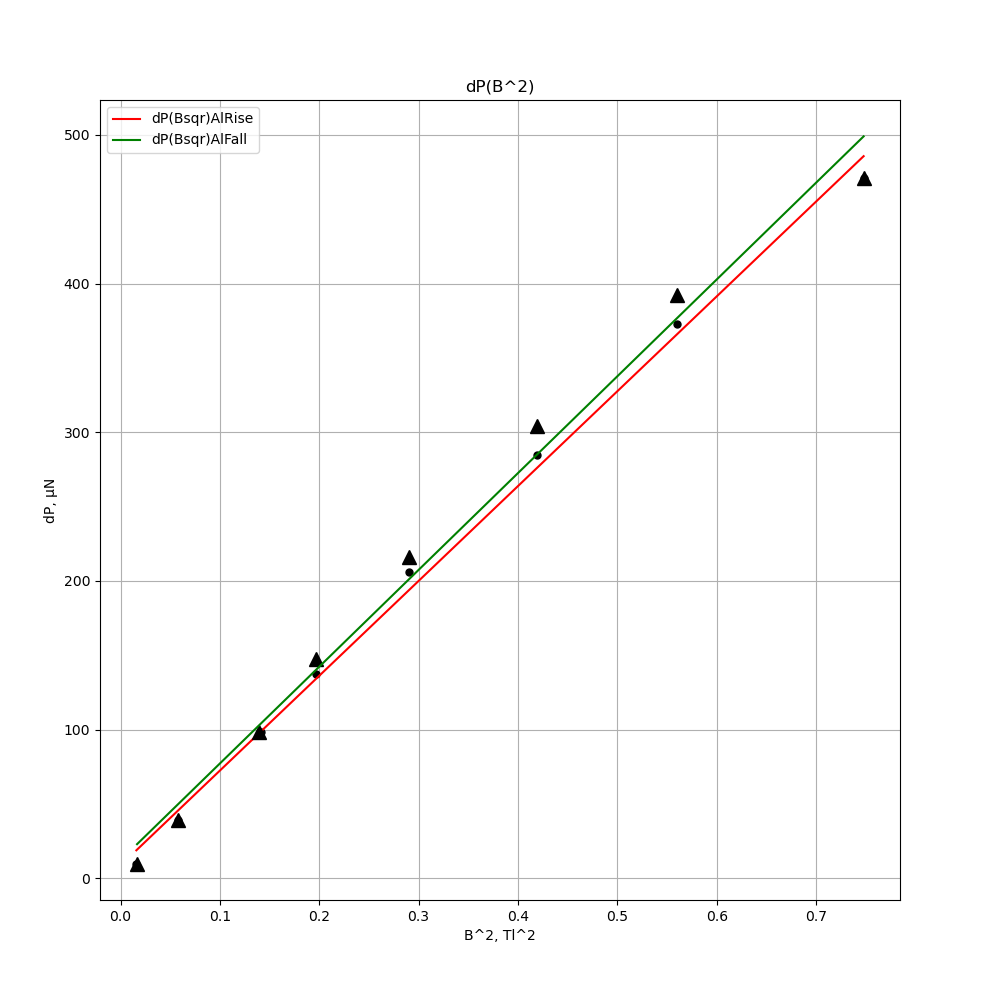
\includegraphics[width=\textwidth]{img/dP(Bsqr)Al.png}
        \caption{Al}
        \label{fig:image3}
    \end{minipage}\hfill
    \begin{minipage}{0.5\textwidth}
        \centering
        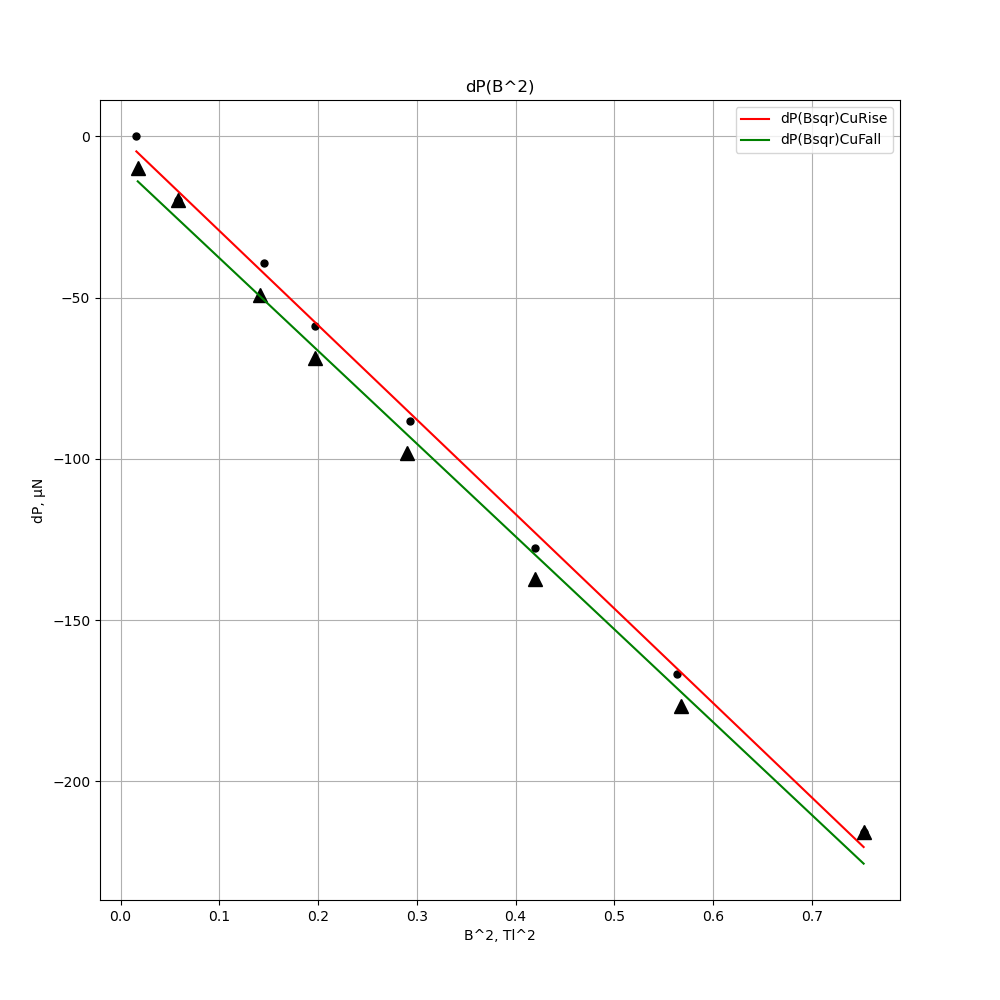
\includegraphics[width=\textwidth]{img/dP(Bsqr)Cu.png}
        \caption{Cu}
        \label{fig:image4}
    \end{minipage}
\end{figure}

Из этих графиков можно найти магнитную восприимчивость наших образцов.

\begin{equation}
    F_M = \diffp*{W_M}{x}{B} = \chi \frac{B^2}{2\mu_0}S = dP
\end{equation}
\begin{equation}
    \alpha = \diffp{F_M}{B}
\end{equation}
\begin{equation}
    \chi = \frac{2\mu_0 \alpha}{S}
\end{equation}

\centering
\subsection*{Вывод}
\raggedright

Таким образом: $\chi_\text{Al} = (2.06 \pm 0.07) \cdot 10^{-6}$,
$\chi_\text{Cu} = (-9.29 \pm 0.25) \cdot 10^{-7}$

Табличные значения: $\chi_\text{Al} = 1.64 \cdot 10^{-6}$,
$\chi_\text{Cu} = -7.71 \cdot 10^{-7}$

Наши измерения отличаются от табличных на $\approx 25\%$. Столь большие отличия
могут быть вызваны большим количеством примясей в образцах. Также мы выяснили,
что медь, в отличие от аллюминия является диамагнетиком и что магнитная восприимчивость
этих материалов крайне мала.

\newpage


\end{document}
